% Encoding: UTF-8
\documentclass[final,bibliography=totocnumbered]{include/sikseminar}

%% Folgende Pakete werden bereits durch die sikseminar-Klasse geladen:
%\usepackage[german]{babel}
%\usepackage[headsepline]{scrlayer-scrpage}
%\usepackage{german}
%\usepackage{graphicx}
%\usepackage{textcomp}
%\usepackage{bibgerm}

\usepackage[utf8]{inputenc}
\usepackage{todonotes}
\usepackage{hyperref}
\usepackage[T1]{fontenc}
\hypersetup{colorlinks = true,linkcolor = black,citecolor = black,urlcolor = black,filecolor = black}
\usepackage[inline]{enumitem}
\usepackage[acronym,toc,section=section,numberedsection,nomain]{glossaries}
\glstoctrue
\makeglossaries
\newacronym[shortplural={CPS},longplural={Cyber-physical Systems}]{cps}{CPS}{Cyber-physical System}


\usepackage[autostyle=true,german=quotes]{csquotes}
\usepackage{subcaption}
\usepackage{xspace}
\graphicspath{{./figure/}}

\usetikzlibrary{shapes.geometric}

\clubpenalty=10000
\widowpenalty=10000


\overfullrule=1mm

\newcommand{\fb}[1]{\dofb#1}
\newcommand{\cps}{\glspl{cps}\xspace}
\newcommand{\dofb}[1]{\textbf{#1}\nobreak\hspace{0pt}}


\begin{document}

\Title[Security Considerations for \glsentrytext{cps}]{Security Considerations for Cyber-Physical Systems}
\makeTitle

\Author{Maximilian Ammann}
\Studiengang{Bachelor Informatik}
\makeAuthor
\date{Datum des Vortrags \todo}
\subject{Seminar Cyber-Physical Systems}

\maketitle

\begin{abstract}
\section*{Kurzfassung}
Eine kurze Zusammenfassung der Ausarbeitung mit 10-12 Zeilen Text.
\end{abstract}
\thispagestyle{empty}
\newpage
\tableofcontents
\newpage

\section{Einführung}\label{sec:intro}
% Anforderungen an CPS: Predictability (Lee08)
% Challanges (SGL+08)
% Vision von CPS (RLS+10)
% IoT Constaint: Battery (YWY+17)
\cps sind meist eingebettete Echtzeitsysteme, welche eine hohe Verfügbarkeit, Robustheit, Widerstandsfähigkeit und Berechenbarkeit aufweisen müssen.
Die physische Welt macht hohe Verfügbarkeit allerdings oft schwierig, da sie alles andere als berechenbar ist~\cite{Lee08,SGL+08}.
Einsatzorte für diese Systeme könnten intelligente Stromnetze, symbiotische Sensornetzwerke für die Agrarwirtschaft und Katastrophenabwehr, medizinische oder assistierende Geräte, intelligente Verkehrssteuerung und intelligente Gebäude sein~\cite{RLS+10}.

In all diesen Beispielen spielt ein außerordentliches Maß an Vertrauen eine Rolle~\cite{SGL+08}.
Dieses ist zwar auch bei Cybersystemen gefordert, allerdings ohne die Koppelung an physische Prozesse~\cite{BG11}.
Zudem unterliegt man konzeptionell bedingt auch einigen Restriktionen wie beispielsweise die Bindung an eine Batterie oder eine leichte Bauweise~\cite{YWY+17}.
Es existiert also ein Unterschied in den Anforderungen an \cps und Cybersystemen, wie Anwendungsservern oder Heimcomputern, sodass man diese in Bezug auf Sicherheit anders betrachten muss.

In dem Kapitel~\ref{sec:bedeutung-sicherheit} wird zunächst das Zusammenspiel von physischen und Cybersystemen im Bezug auch Sicherheit geklärt.
Zudem werden mögliche Ziele und Angreifer in den Kapitel~\ref{subsec:angriffsziel}~und~\ref{subsec:angreifergruppen} beleuchtet.
Im Kapitel~\ref{sec:angriffszenarien} werden mögliche Szenarien und im Kapitel ~\ref{subsec:angreifergruppen} dazu Gegenmaßnahmen dargestellt.
Zuletzt soll im Kapitel~\ref{sec:diskussion} diskutiert werden, ob die genannten Gegenmaßnahmen  für die Szenarien ein adäquate Lösung darstellen.
% Stuxnet (Langer)

% Spectre: https://arxiv.org/pdf/1811.05441.pdf
% EU: https://eur-lex.europa.eu/legal-content/EN/TXT/?uri=JOIN:2017:0450:FIN https://ec.europa.eu/transport/sites/transport/files/3rd-mobility-pack/com20180283_en.pdf


% Encoding: UTF-8

\section{Bedeutung von Sicherheit in \glsentrytext{cps}}\label{sec:bedeutung-sicherheit}

Die Eigenschaften von Cybersystemen und physischen Systemen in Bezug auf Sicherheit unterscheiden sich.
Um Klarheit zu schaffen, wo diese Unterschiede liegen soll Sicherheit speziell für \cps definiert werden.

\subsection{Sicherheitsrelevante Eigenschaften von \glsentrytext{cps}}\label{subsec:definition}
% CIA triad (Fink) (WYX+10)
% Erweiterung von CIA: Veracity, Plausability (Gollman)
Unter Sicherheit bei Cybersystemen versteht man im allgemeinen Informationssicherheit.
Informationssicherheit kann man durch drei Eigenschaften von Systemen charakterisieren~\cite{Cherdantseva2013}:
\begin{itemize}[noitemsep,wide=0pt]
    \item \fb{Confidentiality} - Nur autorisierte Teilnehmer können auf Daten und Ressourcen zugreifen.\label{def:confidentiality}
    \item \fb{Integrity} - Daten und Ressourcen können nur von autorisierten Teilnehmern verändert werden.\label{def:integrity}
    \item \fb{Availability} - Daten und Ressourcen ist für autorisierte Teilnehmer angemessen verfügbar.\label{def:availability}
\end{itemize}

Zwischen diesen drei Eigenschaften muss bei der Entwicklung ein sinnvolles Gleichgewicht gefunden werden.
\citeauthor{GK16} beschreiben, dass bei Cybersystemen der Fokus auf Confidentiality und bei \cps eher auf Availability liegt.
Dieser Fokus ist kritisch zu betrachten, wenn man die diversen Einsatzorte und sicherheitskritischen Anforderungen von \cps betrachtet.

Sie schlagen außerdem vor das CIA-Dreieck im Hinblick auf \cps durch die Eigenschaft Veracity (dt.~Richtigkeit) zu erweitern.
Ein System hat diese Eigenschaft genau dann, wenn Aussagen des Systems die Wahrhaftigkeit der  Wirklichkeit reflektieren.
Es muss also sichergestellt werden, dass Sensoren durch beispielsweise physische Maßnahmen (siehe Kapitel~\ref{subsec:physisch}) fälschungssicher sind.
Confidentiality und Integrity sind nicht ausreichend um die Richtigkeit von Informationen zu garantieren.
Veracity ist eine relativ starke Eigenschaft.
Deshalb kann man in Fällen, in denen diese nur schwer zu erreichen ist, zunächst auf Plausibility setzen.
Herbei hat ein System genau dann diese Eigenschaft, wenn Aussagen des Systems nicht zu weit von erwartbaren Werten abweichen.
Liefert ein Sensor beispielsweise einen für physikalische Modelle unmögliche Wert, so ist dieser nicht plausibel und das System erreicht kann einen möglichen Angriff erkennen. \cite{GK16}
Diese Eigenschaft kann nicht durch Integrity gewährleistet werden, da die Werte eines Sensors von außerhalb beeinflusst werden können.
Veracity stellt also eine grundsätzlich andere Eigenschaft bereit.

\citeauthor{WYX+10} und \citeauthor{SFJ2017} stimmen zu, dass eine Überprüfung auf die Richtigkeit von Informationen wichtig sind.
Sie erweitern das CIA-Dreieck zudem um die Eigenschaft der Authentizität zwischen Kommunikationspartnern.
Authentizität kann hergestellt werden genau dann, wenn sich beide Kommunikationspartner einig über die Identität des Gegenübers sind.\label{def:authenticity}
Obwohl bei der Definition von \citeauthor{Cherdantseva2013} die Authentizität bereits in der Definition beinhaltet ist, soll diese hier dennoch zusätzlich aufgeführt werden.
Es könnte behauptet werden, dass sich Integrity und Authentizität decken.
Daten können allerdings Integrity durch z.B.\ Checksummen und gleichzeitig keine Authentizität besitzen.
In der Realität bringt Authentizität aber oftmals Integrity mit sich.

Ein weiteres wichtiges Konzept ist die Nonrepudiation.
Hierbei darf es nicht möglich sein aufgezeichnete Aktionen zu leugnen \cite{NIST2013}.\todo{Wie zitiert man NIST?}
Ein System hat diese Eigenschaft also genau dann, wenn jegliche Aktionen, die das System beeinflussen, nachvollzogen werden können. \label{def:nonrepudiation}

\begin{figure}
    \centering
    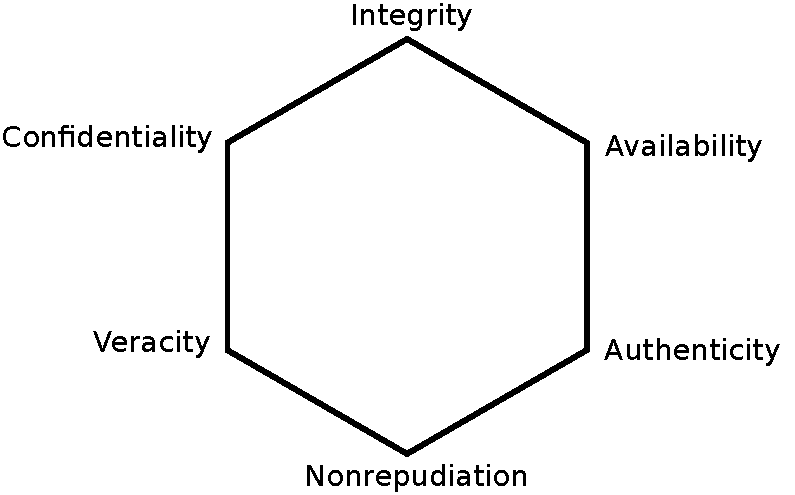
\includegraphics[width=0.5\textwidth]{triad}
    \caption{Erweitertes CIA-Dreieck}
    \label{fig:triad}
\end{figure}

Zusammenfassend kann man sagen, dass die Eigenschaften von Systemen aus der klassischen Informationssicherheit nicht ausreichen um das oft komplexe Zusammenspiel von physischen- und Cybersystemen\todo{physischen- richtig?} abzusichern.
Bei \cps ist also sowohl die Richtigkeit von Informationen als auch die zweifelsfreie Identifikation zweier Parteien wichtig.
Deshalb sind zusätzliche Eigenschaften wie Veracity und Authentizität, wie in Abbildung~\ref{fig:triad} zu sehen ist, nötig um die Aspekte von \cps abzudecken.

% Definition (BG11)
% computer, information, network, communication, physical security
% Fingerprinting, Network Separation, End System Security (Gollman)

\subsection{Angreifergruppen}\label{subsec:angreifergruppen}
% Cyber-Kriminelle
% Verärgerte Mitarbeiter/Private Gründe
% Terroristen, Aktivisten, kriminelle Gruppen
% Staaten (Cardenas 2009, 2.) (WYX+10, II. C.)

Angriffe können von unterschiedlichen Gruppen aus unterschiedlichen Gründen ausgehen.
Im Folgenden sollen verschiedene Gruppen nach den Faktoren
\begin{enumerate*}[label=(\alph*),before=\unskip{: }, itemjoin={{; }}, itemjoin*={{, und }}]
    \item Angreifergruppe\label{factor:angreifergruppe}
    \item Angriffsziel\label{factor:target}
    \item Motiv\label{factor:motiv}
    \item Angriffsvektoren\label{factor:methode}
    \item Konsequenzen\label{factor:konsequenz}
\end{enumerate*} aufgezählt werden~\cite{HLL+17}.\todo{Aufzählung entfernen?}

Kriminelle Gruppen \ref{factor:angreifergruppe} haben oft Erpressung \ref{factor:motiv} als Ziel \cite{WYX+10}.
Dabei sind Cyberangriffe nur ein logischer nächster Schritt der Kriminellen, da diese weitaus günstiger, weniger riskant, nicht durch Entfernungen eingeschränkt und einfacher zu koordinieren und wiederholen sind. \cite{CAS+09}

Computerforensiker~\ref{factor:angreifergruppe} haben nicht unbedingt als Ziel selbst ein System zu beschädigen.
Zum einen kann das Finden von Lücken als Ziel haben, diese unter bestimmten Auflagen offen zulegen oder schließen zu können~\ref{factor:motiv}. \todo{Zitat fehlt}
Zum anderen können diese aber auch als Schadsoftware verkaufen werden~\ref{factor:motiv}. \todo{Zitat fehlt}

Unzufriedene Mitarbeiter~\ref{factor:angreifergruppe} eines Unternehmens haben viel Wissen über dessen Infrastruktur.
Das Motiv kann liegt hierbei bei der Schädigung des Unternehmens~\ref{factor:motiv}.
Zudem existiert eventuell Zugriff auf das System, sodass überhaupt kein Umgehen von Sicherheitsmechanismen notwendig ist~\ref{factor:methode}.~\cite{CAS+09,WYX+10}

Aktivistische Gruppierungen~\ref{factor:angreifergruppe} zielen oft auf kritische \cps~\ref{factor:target}, wie beispielsweise Kernkraftwerke oder \gls{scada} Systemen in Fabriken, ab, um diese zu manipulieren \cite{CAS+09,HLL+17}. \todo{Spionage?}
Damit dies erreicht werden kann existiert die Möglichkeit Forensiker oder Insider zu engagieren~\ref{factor:methode}.~\cite{WYX+10}

Staaten~\ref{factor:angreifergruppe} können politisches und militärisches Interesse~\ref{factor:motiv} daran haben Infrastruktur innerhalb oder außerhalb des Staatsgebiets~\ref{factor:target} anzugreifen \cite{CAS+09}, um diese zu sabotieren oder auszuspionieren.
Auch hier werden Forensiker oder Insider zu engagieren~\ref{factor:methode}.

Das Wissen über den Angreifer und dessen Motivation kann maßgeblich bei der Wahl und der Strategie der Gegenmaßnahmen helfen.
Zudem können dadurch Gefahrenmodelle und detailliertere Angriffsszenarien entworfen werden (siehe Kapitel~\ref{sec:angriffszenarien}).

% Encoding: UTF-8

\section{Angriffsszenarien}\label{sec:angriffszenarien}

\begin{figure}
    \centering
    \begin{subfigure}[b]{0.3\textwidth}
        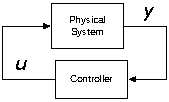
\includegraphics[width=\textwidth]{abstrakt}
        \caption{Ohne Angriffspunkte}
        \label{fig:abstrakt}
    \end{subfigure}
    \qquad
    \begin{subfigure}[b]{0.4\textwidth}
        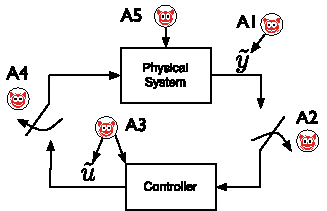
\includegraphics[width=\textwidth]{attack_points}
        \caption{Mit Angriffspunkten}
        \label{fig:attack_points}
    \end{subfigure}
    \caption{Abstraktion eines \cps~\cite{CAS08}}
\end{figure}

In Abbildung~\ref{fig:abstrakt} ist eine abstrakte Darstellung eines \cps zu sehen.
Der \enquote{Controller} sendet Befehle über $u$ an das \enquote{Physical System}.
Dieses wiederum schickt Resultate oder Sensorwerte über $y$ an den \enquote{Controller}.
In Abbildung~\ref{fig:attack_points} sind mögliche Angriffspunkte dargestellt.
Hierbei stellen A1 und A2 Täuschungsangriffe dar, A4 und A2 \gls{dos} und A5 einen physischen Angriff.
Im folgenden Kapitel sollen Angriffe an verschiedenen Punkten eines \cps dargestellt werden.

% Sabotage und Spionage
% Punkte wo angegriffen werden kann (Fink, Figure 1.1) (Cardenas 2008, Figure 3)
% Migration von Legacy Systemen ist kritisch (Gollman, 1.)
% Unterschied zu Cybersystemen (Cardenas 2008, 3.)
% IoT Unterschiede zu Cybersystemen (FPA+18)
% Workflow von CPS (WYX+10, II.)
\subsection{\glsentrytext{dos} Angriff}\label{subsec:dos}
% Availability

\gls{dos} Angriffe zielen darauf ab das Cybersystem mit einer großen Flut an Informationen zu stören.
Diese können von einem angeschlossenes Netzwerk oder dem physischen System ausgehen.
Dadurch wird der Informationsfluss von Steuer- und Nutzdaten, wie in Abbildung~\ref{fig:attack_points} an den Punkten A4 und A2 zu sehen ist, unterbrochen und die Availability des \cps eingeschränkt.

Diese Angriffe sind beispielsweise bei CAN Bussen in Autos realistisch, da Nachrichten mit vielen Empfängern gesendet werden und auch die Fehlerbehebung angreifbar ist~\cite{HUM 81,26}.% HUM 81: Konkret wurde der Tacho auf 0 gesetzt
Folgen können sein, dass sich Fenster nicht mehr schließen lassen, Warnlichter oder die Diebstahlsicherung deaktiviert werden können~\cite{HUM 68}.

Auch in echtzeitkritischen intelligenten Stromnetzen kann ein massives Überfluten dazu führen, dass der Normalbetrieb nicht mehr möglich ist~\cite{HUM 98}.
Der Einsatz von kabelloser Kommunikation erhöht dabei das Angriffspotential~\cite{HUM 99}, da diese allgemein eine geringere Bandbreite aufweisen.
% (WYX+10, II. B.)
% (Cardenas 2008, 2.1)
\subsection{\glsentrytext{mitm} Angriff}\label{subsec:mitm}
% no Authentizität -> Confidentiality, Integrity
% (WYX+10, II. B.)
%Cite http://www.security-science.com/pdf/active-man-in-the-middle.pdf ??
Bei \gls{mitm} Angriffe kann man zwischen aktiven und passiven Angriffen unterscheiden~\cite{WYX+10}.
Passive verändern den Netzwerkverkehr nicht, sondern lauschen nur um an Informationen zu gelangen (siehe Kapitel~\ref{subsec:lauschen}).
Bei aktiven hingegen wird der Verkehr zwischen zwei Kommunikationspartnern zudem noch verändert.
Beide Arten nutzen allerdings dieselben initialen Angriffsvektoren.
In der Abbildung~\ref{fig:attack_points} stellt A1 einen aktiven \gls{mitm} Angriff dar.
Ein Controller kommuniziert über ein Netzwerk mit einem physischen System über die Verbindungen y und u.
Ziel eines Angreifers ist es den Netzwerkverkehr zwischen den beiden anderen Hosts über sich zu leiten~\cite{WYX+10,FPA+18}.
Diese Angriffe können also aufgrund von fehlender Authentizität zu einem Verlust von Confidentiality und Integrity führen.

Dies ist in IEEE 802.11 Netzwerken beispielsweise über ARP-Poisoning möglich~\cite{FIT+2012}.
Aber auch bei Ethernet Verbindungen sind \gls{mitm} Angriffe gängig~\cite{HLL+17}.

Ein weiteres Beispiel für diese Art von Angriffen sind offline Relay Angriffe.
Dabei werden langwellige Signale, welche von Autos an den Schlüssel des Besitzers gesendet werden, um festzustellen, ob dieser in der Nähe ist, abgefangen und aufgezeichnet.
Beim Abspielen dieses Signals, in der Nähe des Besitzers sendet der Schlüssel ein Hochfrequenzsignal, welches wiederum aufgezeichnet wird.
Das Abspielen dieses HF-Signals kann dann genutzt werden, um das Auto aufzuschließen und anschließend zu starten.~\cite{HLL+17}

\subsection{Lauschangriff (Eavesdropping)}\label{subsec:lauschen} % Eavesdropping
% no Authentizität -> Confidentiality
% (WYX+10, II. B.)

\subsection{T\"auschungsangriff (Deception)}\label{subsec:tauschung} % Deception
% no Authentizität -> Integrity
% no Authentizität -> Veracity
% (Cardenas 2008, 2.1)




\subsection{Compromised-Key Angriff}\label{subsec:key}
% Diebstahl -> Nonrepudiation
% (WYX+10, II. B.)

Nonrepudiation kann Aufschluss auf eine solche Attacke geben, da Aktionen getätigt wurden, welche aber nicht von der eigentlich berechtigten Person getätigt wurden.


\todo{Tabelle mit Angriffen und Eigenschaften}

\section{Gegenmaßnahmen}\label{sec:gegenmassnahmen}
% Properties: Safety, Security, Reliability, Resilence (LLZ+14)

% Least Privilege (Gollman)
% Need-to-Know (Gollman)
% Separation (Gollman)

% Proactive Mechanisms, Reactive Mechanisms, Design and Analysis Principles (Cardenas 2008)

% Context Aware Security: Sensing, Cyber, Control, Physical Security (WYX+10)

\subsection{Modellierung von \glsentrytext{cps}}\label{subsec:modellierung}
% Argument: Neue Grundlage für Embedded Systems/CPS: Modelbasiert anstatt Programm (Lee08)
Noch nicht sicher.

Um hierbei dem Standard an Sicherheit zu genügen, schlägt \citeauthor{Lee08} sogar vor eine neue Grundlage für diese Systeme zu etablieren~\cite{Lee08}.

\subsection{Physische Maßnahmen}\label{subsec:physisch}
% (Cardenas)

\subsection{Organisatorische Maßnahmen}\label{subsec:orga}
% Transdiszipliär (Brazell14)
% Betriebsblindheit (Gollman)

\subsection{Präventive Maßnahmen}\label{subsec:präventiv}
% Security by Obscurity (Scarfone2008)
% (Cardenas 2009, 4.)

MITM Angriffen kann mithilfe von Verschlüsselung und Authentizität am besten entgegengewirkt werden.

\subsection{Detektion und Wiederherstellung (Detection and Recovery)}\label{subsec:detektion}
% (Cardenas 2009, 4.)
DoS: rate limiting

\subsection{Widerstandsfähigkeit (Resilience)}\label{subsec:widerstand} % Resilience
% (Cardenas 2009, 4.)

% End-to-End Security (Fink)
DoS: rate limiting

\subsection{Abschreckung (Deterrence)}\label{subsec:abschreckung} % Deterrence
% (Cardenas 2009, 4.)

\section{Sind die Gegenmaßnahmen für potenzielle Szenarien ausreichen?}\label{sec:diskussion}

Sind sie Notwendig?
Ja! -> Sind sie Ausreichend?


\newpage
\printglossary[type=\acronymtype]
~\nocite{*}

\printbibliography
\newpage
% \listoftodos
\end{document}
